\documentclass[conference]{IEEEtran}
\IEEEoverridecommandlockouts
\usepackage[T1]{fontenc}
\renewcommand{\ttdefault}{lmtt}
\usepackage{cite}
\usepackage{amsmath,amssymb,amsthm}
\usepackage{graphicx}
\usepackage{booktabs,array}
\usepackage{xcolor}
\usepackage{tikz}
\usetikzlibrary{positioning,arrows.meta,fit,backgrounds,calc}
\usepackage[hidelinks]{hyperref}
\usepackage{microtype}
\graphicspath{{../artifact/figures/}}
\newtheorem{proposition}{Proposition}
\newtheorem{lemma}{Lemma}
\newcommand{\sys}{ZS-PRISM}
\newcommand{\BCKBQfive}{696\,kB}
\newcommand{\BCKBQfour}{732\,kB}
\newcommand{\CensusFaster}{26\%}
\newcommand{\CensusSlowerClause}{is never slower than}
\newcommand{\CorrQueries}{1{,}000}
\newcommand{\EightMPCQfourWan}{2.69\,s}
\newcommand{\EightMPCQoneWan}{7.82\,s}
\newcommand{\EightZSQfourLan}{289\,ms}
\newcommand{\EightZSQfourWan}{911\,ms}
\newcommand{\EightZSQoneWan}{50.5\,ms}
\newcommand{\IngMap}{90{,}480}
\newcommand{\IngPaillier}{220}
\newcommand{\IngZS}{113{,}192}
\newcommand{\LocalFaster}{15\%}
\newcommand{\LocalSlowerClause}{is never more than 0.04\,ms slower than}
\newcommand{\MPCLocalQfour}{3.51\,ms}
\newcommand{\MPCLookupMillion}{292\,ms}
\newcommand{\MPCQfourTen}{214\,ms}
\newcommand{\MPCQtwoMillion}{61.9\,ms}
\newcommand{\MPCRounds}{10}
\newcommand{\MPCSpeedup}{2.2$\times$}
\newcommand{\MapBootMillion}{903\,ms}
\newcommand{\MapBootThree}{3.28\,s}
\newcommand{\MapHeapMillion}{399\,MB}
\newcommand{\MapHeapPerRec}{399}
\newcommand{\MaxIQR}{5\%}
\newcommand{\MillionIngZS}{35.04\,s}
\newcommand{\MillionQfourZS}{209\,ms}
\newcommand{\MillionScan}{2.02\,s}
\newcommand{\NAdult}{45{,}222}
\newcommand{\PDKBQfive}{13\,kB}
\newcommand{\PDKBQfour}{295\,kB}
\newcommand{\PDSaveQfive}{55.3$\times$}
\newcommand{\PDSaveQfour}{2.5$\times$}
\newcommand{\PaillierSlowdown}{514$\times$}
\newcommand{\ScqlQfourLocA}{57.7\,ms}
\newcommand{\ScqlQfourLocM}{585\,ms}
\newcommand{\ScqlQfourWanA}{755\,ms}
\newcommand{\ScqlQfourWanM}{2.08\,s}
\newcommand{\ScqlQthreeWanM}{103\,ms}
\newcommand{\ScqlRtt}{23.8\,ms}
\newcommand{\ScqlSpeedupMax}{9.3$\times$}
\newcommand{\ScqlSpeedupMin}{2.3$\times$}
\newcommand{\SelQfive}{91}
\newcommand{\SelQfour}{976}
\newcommand{\SelQthree}{18{,}942}
\newcommand{\SelQtwo}{6{,}008}
\newcommand{\SnapRankZS}{0.00\%}
\newcommand{\SnapShareSum}{100\%}
\newcommand{\SnapShared}{100\%}
\newcommand{\SnapZS}{0\%}
\newcommand{\TraceBCClause}{no target is linked (0 of 1{,}000)}
\newcommand{\TraceLinkedPD}{2.0\%--3.2\%}
\newcommand{\TraceSetBC}{4{,}845}
\newcommand{\TraceSetPD}{534}
\newcommand{\UtilMdavAvg}{0.26\%}
\newcommand{\UtilMdavFive}{1.4\%}
\newcommand{\UtilMondFive}{5.2\%}
\newcommand{\UtilMondTail}{64\%}
\newcommand{\WanAdaptiveWin}{1.9$\times$}
\newcommand{\WanAutoBestFrac}{26 of 30}
\newcommand{\WanBChigh}{86.5\,ms}
\newcommand{\WanBClow}{65.5\,ms}
\newcommand{\WanMapWorse}{1.7$\times$}
\newcommand{\WanPDhigh}{267\,ms}
\newcommand{\WanPDlow}{57.3\,ms}
\newcommand{\WanRegret}{0\%}
\newcommand{\WanRegretMax}{25\%}
\newcommand{\WanScan}{527\,ms}
\newcommand{\WanSharedDiff}{2\%}
\newcommand{\WritePaillier}{4.7}
\newcommand{\WriteZS}{0.15/0.16/0.12}
\newcommand{\ZSBoot}{6\,\textmu s}
\newcommand{\ZSLocalQfour}{7.81\,ms}
\newcommand{\ZSLookupMillion}{0.20\,ms}
\newcommand{\ZSQfourTen}{96.7\,ms}
\newcommand{\ZSQfourWanA}{86.4\,ms}
\newcommand{\ZSQthreeWanM}{2.19\,s}
\newcommand{\ZSQtwoMillion}{1.71\,ms}


\begin{document}

\title{ZS-PRISM: Stateless and Unlinkable Record Linkage for Privacy-Preserving Multi-Cloud Data Splitting}

\author{\IEEEauthorblockN{Shivambu Dev Pandey, Sarthak Goyal, Anas Khan, and Mayank Bansal}
\IEEEauthorblockA{Indian Institute of Information Technology Dharwad, India}}

\maketitle

\begin{abstract}
In vertical data splitting, the attributes of a sensitive relation are divided into fragments and each fragment is stored at a different cloud provider, on the assumption that the providers do not collude. When a query needs attributes from several fragments, a proxy has to put the matching records back together. Current designs do this in one of two ways. Some give all fragments of a record the same identifier, so colluding providers can simply join on it. Others keep a linkage map with one entry per record at the proxy, and this map has to be replicated and restored whenever a proxy fails. This paper describes \sys{}, a splitting proxy that needs neither. It has three parts. (C1) \emph{Stateless root-key linkage}: the key of a fragment is an AES permutation of a random row identifier together with the provider index. Such keys cannot be linked across providers, the proxy can invert them, and the proxy stores nothing persistently except a 32-byte root key. (C2) \emph{Dual-share splitting}: the numeric measure is stored as two additive shares at two providers, and an update rewrites both shares, which prevents either provider from learning how the value changed. (C3) \emph{Selectivity-ordered sequential conjunctive execution}: the proxy visits providers in ascending order of predicate cardinality and forwards only the smallest candidate set, and on high-latency links a cost-based probe decides how to proceed. We evaluated \sys{} against seven baselines on two UCI data sets. It returns the exact answer to every query and \LocalSlowerClause{} map-based splitting on one host. At $10^6$ records it replaces the 60\,MB map by 32 bytes, which cuts proxy bootstrap from \MapBootMillion{} to \ZSBoot{}. Compared with broadcast execution it transfers up to \PDSaveQfive{} less data, and in the WAN setting used by SecretFlow-SCQL it answers cross-provider joins \ScqlSpeedupMin{}--\ScqlSpeedupMax{} faster than SCQL. We also report its leakage: the two share holders can link all records if they collude, and query traces let colluding providers link \TraceLinkedPD{} of records after 1,000 queries.
\end{abstract}

\begin{IEEEkeywords}
Cloud data privacy, data splitting, vertical fragmentation, pseudorandom permutation, secret sharing, encrypted databases, multi-cloud.
\end{IEEEkeywords}

% =====================================================================
\section{Introduction}
Suppose a hospital moves its patient table to the cloud. It may accept that a provider sees ages, or diagnoses, or names, but it does not want one provider to see all three for the same patient. Vertical splitting addresses this by distributing the columns over several providers, so that what each of them stores is harmless when taken alone \cite{aggarwal2005two,ciriani2010combining,ganapathy2012distributing}. Since the columns inside a fragment are not encrypted, a provider can build indexes on them and answer SQL in the usual way. In their survey, Domingo-Ferrer \emph{et al.} compare splitting with anonymization and with cryptographic techniques, and conclude that splitting is the option under which data remain directly queryable at a moderate cost \cite{domingo2019survey}. This holds as long as a query stays within one fragment. For a query over several fragments, the proxy placed between the application and the providers must find out which rows at the different providers belong to the same record.

We call this information \emph{linkage}. Two ways of providing it are known, and each has a drawback. In the first, the fragments of a record all store the same tuple identifier \cite{aggarwal2005two}. The proxy then keeps no state, but two providers that collude, or whose snapshots are leaked together, only need to join their tables on the identifier to reverse the split. In the second, every fragment is stored under an unrelated random key. Now the tables cannot be joined, but the proxy has to store, for every record, the keys that belong together. The survey already warns that this metadata is a single point of failure, because the outsourced data cannot be reconstructed without it, and recommends redundancy and backups \cite[Sec.~3.1.1]{domingo2019survey}. In practice the map has one entry per record, all proxy replicas must agree on it, and a replacement proxy has to load it completely before it can answer its first cross-fragment query.

Our starting point was the question of whether the proxy needs this map at all. In \sys{} it does not, because the proxy \emph{computes} the fragment key of row $r$ at provider $c$ as $h_{r,c}=\mathrm{AES}_{K}(r\Vert c)$. To anyone without $K$ this value looks random, while the proxy can decrypt it and recover $r$. Row identifiers are random and the shares of the measure are drawn fresh, so the proxy has to persist only one 32-byte secret, whatever the number of records $N$, and several replicas can work side by side without coordinating.

\noindent\textbf{Contributions.} This paper contributes the following.
\begin{itemize}
  \item \textbf{C1, stateless root-key linkage.} A fragment key is the AES encryption of a (row, provider) pair under a subkey of a single root key. From a handle returned by a provider, the proxy recovers the row, verifies which provider the handle belongs to, and computes the handle of the same row at any other provider. A linkage map is therefore not needed, the persistent state is a 32-byte secret, and snapshots stored at different providers cannot be linked (Section~\ref{sec:c1}).
  \item \textbf{C2, dual-share splitting.} We store the numeric measure as two additive shares at two providers, and every update replaces both of them, which hides the size of the change from each provider. The providers can add up their own shares, so the proxy receives a single value per provider for an aggregate (Section~\ref{sec:c2}).
  \item \textbf{C3, selectivity-ordered sequential conjunctive execution.} The proxy first asks each provider how many rows match its predicate and then visits the providers starting with the smallest result, translating handles with C1 on the way. If a result is small enough that sending it is cheaper than a further round trip, the provider returns it together with the count (Section~\ref{sec:query}).
  \item An implementation in which each server runs as its own process behind an emulated wide-area link. We compare with seven baselines, namely shared-identifier splitting, map-based splitting, DET+Paillier, DET+AEAD, an AEAD scan, three-party replicated secret sharing and the released SecretFlow-SCQL system, and with MDAV and Mondrian as anonymization methods (Section~\ref{sec:impl}).
  \item An evaluation on two real data sets. It covers correctness, proxy state and failover, latency on one host and over wide-area links, writes, and the utility of anonymization, and it includes two collusion attacks that show what \sys{} does \emph{not} protect (Section~\ref{sec:eval}).
\end{itemize}
Section~\ref{sec:related} discusses related work and Section~\ref{sec:model} states the system and threat model. The three contributions are described in Section~\ref{sec:design}. Sections~\ref{sec:impl} and~\ref{sec:eval} cover the implementation and the experiments, and Section~\ref{sec:disc} discusses limitations.

% =====================================================================
\section{Background and Related Work}\label{sec:related}

\textbf{Data splitting and fragmentation.}
Vertical partitioning over two servers goes back to Aggarwal \emph{et al.} \cite{aggarwal2005two}. In their scheme both fragments contain the tuple identifier, and a sensitive attribute may also be encoded so that each server holds one part of it. The associated optimization problem was studied by Ganapathy \emph{et al.} \cite{ganapathy2012distributing}. Their encoding of a sensitive attribute is a one-time pad over the two servers, which corresponds to the sharing in C2 without updates. Ciriani \emph{et al.} support more than two fragments and make them unlinkable \cite{ciriani2010combining}. Each of their fragments contains all attributes, in clear where this is allowed and encrypted otherwise. A query therefore never joins fragments, but the client has to decrypt, and a variant keeps a small fragment at the data owner \cite{ciriani2009keep}. The splitting workflow in the survey, in contrast, joins fragments across providers. The proxy is then the only party that knows which fragments belong together, and the survey asks for this metadata to be replicated and backed up \cite[Sec.~3.1.1]{domingo2019survey}. Other work publishes a limited amount of linkage on purpose as loose associations \cite{decapitani2010loose}, or considers dependencies in the data through which fragments could be linked again \cite{decapitani2014dependencies}. We do not propose a new fragmentation. \sys{} accepts any fragmentation and only changes the way fragments are linked and queried.

\textbf{Encrypted databases.}
A second line of work encrypts the data and still supports SQL. Examples are bucketization \cite{hacigumus2002executing}, CryptDB with its deterministic, order-preserving and Paillier layers \cite{popa2011cryptdb,bellare2007det,paillier1999}, and Seabed \cite{papadimitriou2016seabed}. These schemes reveal frequencies and order, and inference attacks make use of that \cite{naveed2015inference}. Arx was designed to avoid this leakage and is more expensive \cite{poddar2019arx}. Searchable and structured encryption \cite{kamara2018sql} reveals access patterns, for which generic attacks exist \cite{kellaris2016generic}. In SEAL the amount of such leakage can be adjusted, also for joins \cite{demertzis2020seal}, and d-DSE hides result volumes \cite{liu2024ddse}. For dynamic schemes it is known that less leakage requires more client state \cite{demertzis2020small}. The proxy map that we remove is client state of this kind, used for linkage. Stronger protection is available at higher cost. HE$^3$DB executes filters, aggregates, sorting and joins under fully homomorphic encryption \cite{bian2023he3db}, HEDB runs an encrypted DBMS inside confidential VMs \cite{li2023hedb}, and ORAM conceals access patterns with polylogarithmic overhead \cite{stefanov2013path}.

\textbf{Secret sharing and distributed trust.}
Among systems based on secret sharing, S$^2$ has the trust model most similar to ours \cite{sharma2023s2}. Its non-colluding servers store additive and multiplicative shares. It supports conjunctive, disjunctive and range selections and returns the matching rows, the servers do not talk to each other, and neither the access pattern nor the result size is revealed. Obscure computes aggregates on secret-shared data \cite{gupta2019obscure}. Sharemind, Senate and Secrecy are MPC systems for analytics on shares \cite{bogdanov2008sharemind,poddar2021senate,liagouris2023secrecy}. SecretFlow-SCQL is an MPC SQL platform that is used in production by data owners who collaborate \cite{fang2024scql}. It obtains correlated randomness from a trusted party, and the owners specify which intermediate results may become visible. Alchemy is an optimizer for oblivious SQL plans \cite{sohn2025alchemy}. Every one of these systems protects more than \sys{}. The cost is that a query must process all records or use oblivious operators. \sys{} lets each provider evaluate its predicates on clear data and secret-shares only the measure.

\textbf{Anonymization.}
Methods such as $k$-anonymity \cite{sweeney2002k} and microaggregation \cite{domingo2005ordinal} publish a masked version of the data, on which queries return approximate results. We include MDAV and Mondrian \cite{lefevre2006mondrian} to compare utility. Table~\ref{tab:related} summarizes all families. Its columns give the number of servers and the trust placed in them, the leakage of a server's stored data, the additional leakage during query processing, and the state that the proxy keeps in order to link fragments.

\begin{table*}[t]
\centering
\caption{Comparison of design families for outsourced relational queries.}
\label{tab:related}
\scriptsize
\setlength{\tabcolsep}{3pt}
\begin{tabular}{@{}>{\raggedright\arraybackslash}p{34mm}>{\raggedright\arraybackslash}p{11mm}>{\raggedright\arraybackslash}p{24mm}>{\raggedright\arraybackslash}p{29mm}>{\raggedright\arraybackslash}p{27mm}>{\raggedright\arraybackslash}p{19mm}>{\raggedright\arraybackslash}p{18mm}@{}}
\toprule
Design family & Servers & Trust assumption & Stored-data leakage & Query leakage & Linkage state & Cost evidence\\
\midrule
Shared-TID split \cite{aggarwal2005two,ganapathy2012distributing} & $\ge 2$ & non-colluding & fragments, common tuple ID & access pattern, volume & none & measured \\
Proxy-linked split \cite{domingo2019survey} & $\ge 2$ & non-colluding & fragments & access pattern, volume & $O(N)$ & measured \\
Fragmentation + encryption \cite{ciriani2010combining,ciriani2009keep} & $\ge 1$ & honest-but-curious & fragments, ciphertexts & access pattern, volume & n/a & -- \\
DET/HOM onions \cite{popa2011cryptdb,papadimitriou2016seabed} & 1 & honest-but-curious & equality, order & access pattern, volume & n/a & measured \\
Leakage-adjustable EDB \cite{demertzis2020seal,liu2024ddse} & 1 & honest-but-curious & ciphertexts & adjustable & n/a & published \\
FHE database \cite{bian2023he3db} & 1 & honest-but-curious & ciphertexts & none & n/a & published \\
Confidential-computing DB \cite{li2023hedb} & 1 & trusted hardware & ciphertexts & enclave-dependent & n/a & published \\
Secret-shared outsourcing \cite{sharma2023s2,gupta2019obscure} & $\ge 4$ & non-colluding & shares & none & n/a & published \\
MPC SQL \cite{fang2024scql,liagouris2023secrecy,sohn2025alchemy,bogdanov2008sharemind,poddar2021senate} & 2--3 & semi-honest & shares & declared intermediates (SCQL) & n/a & measured, published \\
Anonymized release \cite{lefevre2006mondrian,domingo2005ordinal} & any & none & masked values & none & n/a & measured \\
\textbf{\sys{} (this work)} & 3 & non-colluding share holders & fragments, one share each$^{\dagger}$ & access pattern, volume, handle traces & $O(1)$ (32\,B root key) & measured \\
\bottomrule
\end{tabular}\\[2pt]
\raggedright\scriptsize Linkage state: what the proxy persists to relate fragments of one record; n/a for designs without fragments. $^{\dagger}$Both share holders together can link and reconstruct records (Section~\ref{sec:attacks}).
\end{table*}

% =====================================================================
\section{System and Threat Model}\label{sec:model}
\textbf{Parties.} We trust the data owner, its applications and the \emph{proxy}, through which all operations pass and of which several replicas may exist. There are $m=3$ storage providers $S_0,S_1,S_2$ that belong to different organizations. Each provider stores one fragment and offers a SQL interface to it (Fig.~\ref{fig:arch}).

\textbf{Data and fragmentation.} A record consists of a direct identifier, several quasi-identifiers (QIs), a sensitive attribute and a numeric measure. For Adult \cite{adult1996} we store \texttt{age, sex} at $S_0$, \texttt{education, marital} at $S_1$, and \texttt{occupation, race, country} at $S_2$. With this placement a provider sees at most two of the six QIs, and the sensitive attribute \texttt{occupation} is stored at a different provider than the identifier. $S_0$ holds the identifier only in the form of a keyed token. The measure, \texttt{hours-per-week}, is not stored anywhere in clear: $S_0$ and $S_1$ each hold one additive share of it. We do not address how a fragmentation should be derived from confidentiality constraints, which has been studied separately \cite{ciriani2010combining,ganapathy2012distributing}. \sys{} can be used with any fragmentation.

\textbf{Adversary.} We assume honest-but-curious providers. A provider answers every request correctly, and it remembers its fragment, the predicates it was asked to evaluate, and all handles that it received or returned. Providers may form coalitions and combine their \emph{snapshots} (the stored tables) or their \emph{traces} (the request logs). Attacks on the network are prevented by TLS. Providers that return wrong results are outside our model, and authenticated data structures \cite{li2006authenticated} would be needed to detect them.

\textbf{Goals.} (G1) Supported queries return exact answers. (G2) The proxy keeps no persistent state per record. (G3) A coalition that lacks at least one share holder cannot link stored data across providers. (G4) The cost stays within a small factor of a design that uses the same placement and a linkage map. Access patterns, result sizes and the clear values in a provider's own fragment remain visible, as in other splitting systems. Section~\ref{sec:attacks} quantifies the linkage that follows from them.

\textbf{Workflow.} Fig.~\ref{fig:arch} shows both paths through the system. To ingest a record (I), the proxy chooses a row identifier $r$ and computes the handles $h_{r,0},h_{r,1},h_{r,2}$ (C1). It then substitutes a keyed token for the identifier, divides the measure into the shares $s_0$ and $s_1$ (C2), and stores one fragment at each provider. A query (C3) takes the following steps. \textcircled{\scriptsize 1} The application sends the query to the proxy. \textcircled{\scriptsize 2} Each provider receives its predicate $\phi_c$ from the proxy. \textcircled{\scriptsize 3} The provider answers with the cardinality $c_c$ and, if $c_c\le\tau_c$, with the matching rows. \textcircled{\scriptsize 4} The proxy inverts the handles and translates them. \textcircled{\scriptsize 5} The candidates go to the next provider, in ascending order of $c_c$. \textcircled{\scriptsize 6} That provider returns its matches together with shares, or with a modular sum of shares. \textcircled{\scriptsize 7} The proxy sends the result to the application. During all of this the only persistent data at the proxy is $K$, and a provider never learns the identifier, the measure, or the handles used at another provider.

\begin{figure*}[t]
\centering
\resizebox{\textwidth}{!}{% Fig. 1 -- ZS-PRISM architecture with numbered query workflow (TikZ)
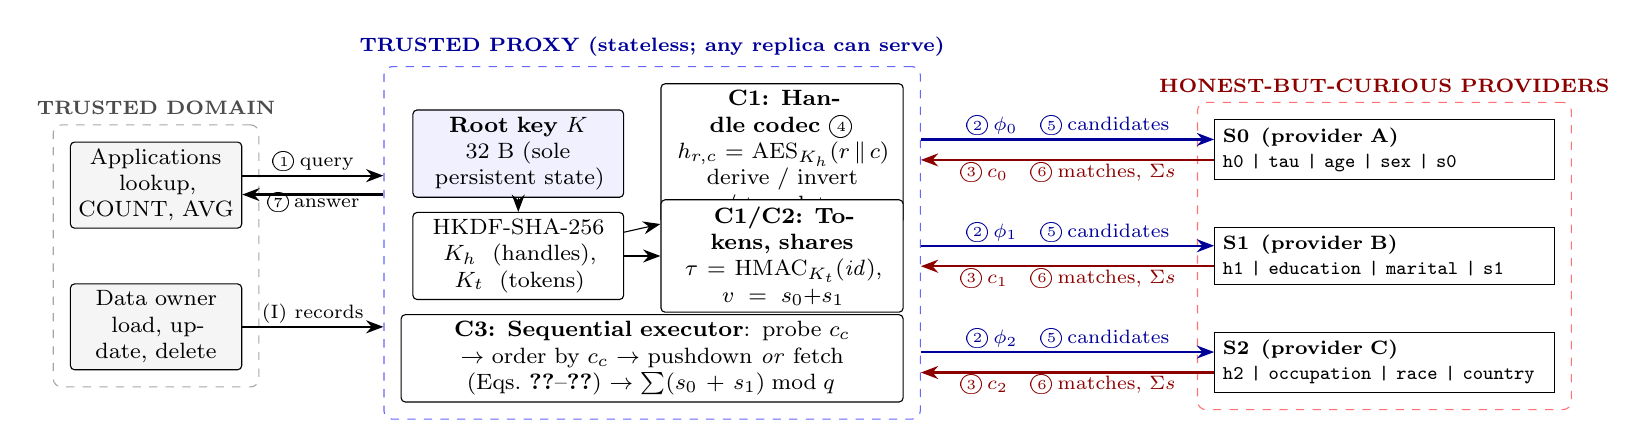
\begin{tikzpicture}[
  font=\footnotesize,
  >={Stealth[length=2.2mm]},
  comp/.style={draw, rounded corners=1.5pt, fill=white, align=center, minimum height=8mm, inner sep=2.5pt, text width=#1},
  comp/.default=26mm,
  zone/.style={draw, dashed, rounded corners=3pt, inner sep=6pt},
  tbl/.style={draw, fill=white, align=left, inner sep=3pt, text width=41mm, font=\scriptsize},
  lbl/.style={font=\scriptsize, align=center, inner sep=1pt},
  flow/.style={->, thick},
]
% ---------------- trusted domain
\node[comp=20mm, fill=gray!8] (app) at (0,0.55) {Applications\\ lookup, COUNT, AVG};
\node[comp=20mm, fill=gray!8] (own) at (0,-1.25) {Data owner\\ load, update, delete};

% ---------------- proxy
\node[comp=25mm, fill=blue!6] (key) at (4.6,0.95) {\textbf{Root key} $K$\\ 32 B (sole persistent state)};
\node[comp=25mm] (hkdf) at (4.6,-0.35) {HKDF-SHA-256\\ $K_h$ \ (handles), \ $K_t$ \ (tokens)};
\node[comp=29mm] (prp) at (7.95,0.95) {\textbf{C1: Handle codec} \textcircled{\tiny 4}\\ $h_{r,c}=\mathrm{AES}_{K_h}(r\,\Vert\,c)$\\ derive / invert / translate};
\node[comp=29mm] (tok) at (7.95,-0.35) {\textbf{C1/C2: Tokens, shares}\\ $\tau=\mathrm{HMAC}_{K_t}(\mathit{id})$,\ \ $v=s_0{+}s_1$};
\node[comp=62mm] (plan) at (6.3,-1.65) {\textbf{C3: Sequential executor}: probe $c_c$ $\rightarrow$ order by $c_c$ $\rightarrow$ pushdown \emph{or} fetch (Eqs.~\ref{eq:bc}--\ref{eq:cost}) $\rightarrow$ $\sum (s_0+s_1) \bmod q$};
\draw[->] (key) -- (hkdf);
\draw[->] (hkdf) -- (prp.south west);
\draw[->] (hkdf) -- (tok);
\node[zone, draw=blue!60, fit=(key)(hkdf)(prp)(tok)(plan), label={[font=\scriptsize\bfseries, text=blue!60!black]above:TRUSTED PROXY (stateless; any replica can serve)}] (pz) {};
\node[zone, draw=gray!70, fit=(app)(own), label={[font=\scriptsize\bfseries, text=gray!60!black]above:TRUSTED DOMAIN}] (cz) {};

% ---------------- providers
\node[tbl] (s0) at (15.6,1.0)  {\textbf{S0 \,(provider A)}\\[1pt]\texttt{h0 | tau | age | sex | s0}};
\node[tbl] (s1) at (15.6,-0.35){\textbf{S1 \,(provider B)}\\[1pt]\texttt{h1 | education | marital | s1}};
\node[tbl] (s2) at (15.6,-1.7) {\textbf{S2 \,(provider C)}\\[1pt]\texttt{h2 | occupation | race | country}};
\node[zone, draw=red!55, fit=(s0)(s1)(s2), label={[font=\scriptsize\bfseries, text=red!55!black]above:HONEST-BUT-CURIOUS PROVIDERS}] (sz) {};

% ---------------- flows (circled numbers: order of one conjunctive query)
\newcommand{\sn}[1]{\textcircled{\tiny #1}}
\draw[flow] ([yshift=1.2mm]app.east) -- ([yshift=1.2mm]pz.west |- app.east) node[midway, above, lbl]{\sn{1}\,query};
\draw[flow] ([yshift=-1.2mm]pz.west |- app.east) -- ([yshift=-1.2mm]app.east) node[midway, below, lbl]{\sn{7}\,answer};
\draw[flow] (own.east) -- (pz.west |- own.east) node[midway, above, lbl]{(I) records};
\foreach \s/\c in {s0/0, s1/1, s2/2} {
  \draw[flow, blue!60!black] ([yshift=1.3mm]pz.east |- \s.west) -- ([yshift=1.3mm]\s.west)
    node[midway, above, lbl, text=blue!60!black]{\sn{2}\,$\phi_{\c}$\quad \sn{5}\,candidates};
  \draw[flow, red!55!black] ([yshift=-1.3mm]\s.west) -- ([yshift=-1.3mm]pz.east |- \s.west)
    node[midway, below, lbl, text=red!55!black]{\sn{3}\,$c_{\c}$\quad \sn{6}\,matches, $\Sigma s$};
}
\end{tikzpicture}
}
\caption{\sys{} architecture: ingestion path (I) and query path (1)--(7).}
\label{fig:arch}
\end{figure*}

% =====================================================================
\section{Design}\label{sec:design}
We use one record as an example throughout this section. Its fragments are \texttt{(38, F)} at $S_0$, \texttt{(Bachelors, Married)} at $S_1$, and \texttt{(Exec-managerial, \dots)} at $S_2$. The proxy stores a \emph{root key} $K$ of 32 bytes. Two subkeys are derived from it with HKDF-SHA-256 \cite{rfc5869} under different labels, $K_h=\mathrm{HKDF}(K,\textit{handle})$ for handles and $K_t=\mathrm{HKDF}(K,\textit{token})$ for identifier tokens. The proxy has no other persistent data. It keeps neither a row map nor a row counter, and it does not track update epochs. The symbols used below are collected in Table~\ref{tab:notation}.

\begin{table}[t]
\centering
\caption{Notation.}
\label{tab:notation}
\scriptsize
\begin{tabular}{@{}ll@{}}
\toprule
Symbol & Meaning\\
\midrule
$N$, $m$ & number of records; number of providers ($m=3$)\\
$K$, $K_h$, $K_t$ & root key; handle and token subkeys\\
$r$ & 96-bit row identifier\\
$E_K$ & AES-256 block encryption under key $K$\\
$h_{r,c}$ & handle of row $r$ at provider $S_c$\\
$T_{c\to c'}$ & handle translation from $S_c$ to $S_{c'}$\\
$v$; $s_0,s_1$ & numeric measure; its additive shares\\
$q$ & share modulus, $2^{61}-1$\\
$\phi_c$; $c_c$ & predicate at $S_c$; its cardinality\\
$\rho$, $B$ & round-trip time; link rate\\
$\beta_c$ & cost of moving one result row from $S_c$\\
$\tau_c$ & threshold for returning rows inline\\
\bottomrule
\end{tabular}
\end{table}

\subsection{C1: Stateless root-key linkage}\label{sec:c1}

When a record is inserted, the proxy draws a new row identifier $r\in\{0,1\}^{96}$ from the OS CSPRNG. Provider $c$ stores its fragment of the record under the handle
\begin{equation}
  h_{r,c} = E_{K_h}\big(r \,\Vert\, \langle c\rangle_{32}\big) \in \{0,1\}^{128}.
  \label{eq:handle}
\end{equation}
$E$ denotes AES-256 on one block \cite{fips197}, which we treat as a pseudorandom permutation (PRP) \cite{luby1988prp}. The input $r\Vert\langle c\rangle_{32}$ is 128 bits long and thus occupies one block, so we need neither a mode of operation nor format-preserving encryption. When $S_c$ returns a handle $h$, the proxy decrypts it,
\begin{equation}
  (r,\,c') = E^{-1}_{K_h}(h)\ \text{ split as } 96\,|\,32 \text{ bits},
  \label{eq:invert}
\end{equation}
and accepts it only if $c'=c$. A handle taken from one provider and replayed at another is rejected by this check. To address the same row at a different provider $c'$, the proxy applies the translation
\begin{equation}
  T_{c\to c'}(h) = E_{K_h}\big(r \,\Vert\, \langle c'\rangle_{32}\big),
  \label{eq:translate}
\end{equation}
where $r$ comes from Eq.~(\ref{eq:invert}). In the example, $h_{r,0}$, $h_{r,1}$ and $h_{r,2}$ are 16-byte strings with no visible relation. If $S_2$ reports a match, the proxy obtains $h_{r,1}$ with one AES decryption and one AES encryption and does not look anything up. Two random 96-bit identifiers coincide with probability at most $N^2/2^{97}$, which is less than $10^{-17}$ for $N=10^6$. Replicas of the proxy can therefore insert records at the same time without agreeing on identifiers. We cluster every fragment table on the handle (SQLite \texttt{WITHOUT ROWID}), so the physical order of rows contains no information other than the handle.

\begin{proposition}[Snapshot unlinkability]
Let $\mathcal{C}\subseteq\{S_0,S_1,S_2\}$ be a coalition that does not contain both share holders. If $E$ is a secure PRP, the joint distribution of the coalition's stored tables is computationally indistinguishable from one in which the rows of each fragment are independently and uniformly permuted, conditioned on their clear-text columns.
\end{proposition}
\begin{IEEEproof}[Proof sketch]
Replace $E_{K_h}$ by a random permutation $\pi$; any distinguisher between the two worlds breaks the PRP. Under $\pi$, the values $\pi(r\Vert c)$ for distinct inputs are uniform distinct strings, independent of the clear-text columns; distinct $c$ give distinct inputs even for the same $r$, so each fragment's handle column is a uniformly random relabelling that is independent across providers. A coalition holding at most one share sees only uniformly random values in $\mathbb{Z}_q$, independent of all other columns. Identifier tokens appear at $S_0$ only.
\end{IEEEproof}
The restriction on the coalition cannot be dropped. For two shares of one row, $s_0+s_1 \bmod q$ lies in $[1,99]$. For two shares of different rows this happens with probability of about $2^{-54}$. $S_0$ and $S_1$ can use this test to link all records and reconstruct the measure (Section~\ref{sec:attacks}). Any 2-out-of-2 sharing of a value from a small range has this property, and for this reason the two shares are given to providers that we assume do not collude.

The direct identifier is kept at $S_0$ and nowhere else, in the form of a keyed token \cite{rfc2104}
\begin{equation}
  \tau = \mathrm{HMAC}_{K_t}(\mathit{id})\ \text{truncated to 128 bits}.
  \label{eq:token}
\end{equation}
$S_0$ can index the token and find a record by exact match. The only thing it learns is whether two identifiers are equal, and no other provider learns even that.

\subsection{C2: Dual-share splitting with refresh}\label{sec:c2}
For the measure $v$ the proxy creates two additive shares, one for $S_0$ and one for $S_1$:
\begin{equation}
  s_0\xleftarrow{\$}\mathbb{Z}_q,\qquad s_1=(v-s_0)\bmod q,\qquad q=2^{61}-1.
  \label{eq:split}
\end{equation}
The value is reconstructed as $v=(s_0+s_1)\bmod q$. As a small example with modulus 101, let $v=37$ and let the mask be $s_0=80$. Then $s_1=58$, and indeed $(80+58)\bmod 101=37$. Consider now an update from $v$ to $v'$. If the proxy kept the mask and replaced only $s_1$, then $S_1$ could compute $s_1'-s_1=v'-v$ and would know the change exactly. With \emph{dual-share refresh} the proxy chooses a new mask for each update and writes two new shares:
\begin{equation}
  s_0'\xleftarrow{\$}\mathbb{Z}_q,\qquad s_1'=(v'-s_0')\bmod q.
  \label{eq:refresh}
\end{equation}
\begin{lemma}[Update privacy]
Let a value change from $v$ to $v'$, with masks $s_0,s_0'\xleftarrow{\$}\mathbb{Z}_q$ drawn independently before and after the update. For each $c\in\{0,1\}$, the pair $(s_c,s_c')$ observed by $S_c$ is uniform on $\mathbb{Z}_q^2$ and hence independent of $(v,v')$.
\end{lemma}
\begin{IEEEproof}
$(s_0,s_0')$ is uniform by construction. For $S_1$, the map $(s_0,s_0')\mapsto(v-s_0,\,v'-s_0')$ is a bijection of $\mathbb{Z}_q^2$ for any fixed $(v,v')$, so $(s_1,s_1')$ is uniform as well. Without refresh ($s_0'=s_0$), $s_1'-s_1=v'-v$ reveals the change.
\end{IEEEproof}
The mask could also be computed as a PRF of the row identifier and an update epoch. In that case the proxy would have to persist the epoch and guarantee that it never goes back. We avoid this because both shares are stored at the providers and the proxy has no reason to recompute an old mask. It takes the mask from the OS CSPRNG, no epoch is needed, and the persistent state remains 32 bytes. For aggregates, $S_0$ and $S_1$ each provide a modular-sum function. Given a candidate set $C$, the proxy asks a share holder for
\begin{equation}
  \sigma_c(C)=\sum_{r\in C} s_{c,r} \bmod q
  \label{eq:agg}
\end{equation}
and gets back 8 bytes, where it would otherwise receive $|C|$ shares. From the provider's point of view this sum is uniformly distributed. For an update or a deletion, the proxy looks up the token at $S_0$ to obtain $r$ and then issues the writes to the providers in parallel. A deployment has to make a write that affects two providers atomic. Two-phase commit or Paxos commit can be used for this without modification \cite{gray2006consensus}.

\subsection{C3: Selectivity-ordered sequential conjunctive execution}\label{sec:query}
We consider conjunctive queries $\sigma_{\phi_0\wedge\phi_1\wedge\phi_2}$, possibly with \texttt{COUNT} or \texttt{AVG}. The proxy splits the condition into one predicate $\phi_c$ per provider. If all predicates refer to the same fragment, that provider answers the query alone. In the other case there are two well-known plans, which Fig.~\ref{fig:seq} illustrates for Q4 (Table~\ref{tab:workloads}). In Q4, $\phi_0$ is a condition on age, $\phi_1$ on education and $\phi_2$ on occupation, and $T_{c\to c'}$ in the figure is the translation of Eq.~(\ref{eq:translate}), which the proxy performs. Under \emph{broadcast}, all providers receive their predicate at once, and the proxy intersects the row identifiers that come back. This takes one round trip. The transferred data, however, grow with $\sum_c c_c$, where $c_c=|\sigma_{\phi_c}|$ is the number of rows matching $\phi_c$. Under \emph{selectivity-ordered semi-join pushdown} \cite{bernstein1981semijoin}, the proxy starts by asking every provider for $c_c$. The provider with the smallest $c_c$ evaluates its predicate first. The proxy inverts the handles it receives (C1), translates them, and sends them as candidates to the provider with the next larger $c_c$, and so on. The transferred data now grow with $c_{\min}$. In exchange, the plan needs a round trip for each provider and one more for the probe. Which provider comes first depends on the query and is not fixed by the schema. Q4 is processed in the order $S_2\to S_1\to S_0$, since the occupation predicate matches the fewest rows, and Q5 in the order $S_0\to S_1\to S_2$, since few rows satisfy its age and sex conditions. A share holder sends its shares along with the handles. If a share holder has no predicate in the query, it is asked for a modular sum in a last round.

\textbf{Cost model.} We write $\rho$ for the round-trip time, $B$ for the link rate and $w_c$ for the number of bytes of a result row from $S_c$. Processing one handle costs $\alpha_s$ at a provider and $\alpha_p$ at the proxy. One result row then costs $\beta_c=w_c/B+\alpha_s+\alpha_p$. Let the providers be sorted so that $c_{(1)}\le\dots\le c_{(m)}$. We estimate the intermediate result sizes as $n_1=c_{(1)}$ and $n_i=n_{i-1}c_{(i)}/N$, which assumes independent attributes in the manner of System R \cite{selinger1979access}. The costs of the two plans are
\begin{align}
 T_{\mathrm{BC}} &= \rho + \textstyle\max_{c}\, c_c\beta_c,\label{eq:bc}\\
 T_{\mathrm{PD}} &= \rho + n_1\beta_{(1)} + \textstyle\sum_{i=2}^{m}\big(\rho + n_{i-1}\beta_{\mathrm{H}} + n_i\beta_{(i)}\big),\label{eq:pd}
\end{align}
with $\beta_{\mathrm{H}}$ the cost of pushing one 16-byte handle. Pushdown needs $m-1$ more round trips than broadcast and is faster only if the data it saves are worth more than $(m-1)\rho$. On links with a large RTT this is often not the case (Section~\ref{sec:wan}), and for this reason \sys{} does not always push down.

\textbf{Adaptive execution.} In \sys{} the probe and the first round are one message. A provider always returns $c_c$. It adds the matching rows if $c_c\le\tau_c$, with the threshold
\begin{equation}
 \tau_c = \hat{\rho}/\beta_c .
 \label{eq:cost}
\end{equation}
Rows are thus included whenever transferring them is cheaper than a further round trip. The proxy maintains $\hat{\rho}$ as an exponentially weighted moving average (EWMA) of observed round-trip times and calibrates $\alpha_s$ and $\alpha_p$ once when it starts. When the probe returns, the proxy knows all cardinalities exactly and has already intersected the results that were included. For the providers that are still missing it evaluates Eqs.~(\ref{eq:bc}) and~(\ref{eq:pd}), beginning from the current intersection, and uses the cheaper of pushdown and a single parallel fetch. If the RTT is high, all results arrive with the probe and the query finishes after one round. If it is low, hardly any result is included and the plan is the same as classical pushdown. The values $\hat{\rho}$ and $\alpha$ and a cached relation size are not persisted. After a restart the proxy measures them again.

\begin{figure}[t]
\centering
\resizebox{\columnwidth}{!}{% Fig. 2 -- message sequence of a three-predicate AVG query (TikZ).
% Every message label sits in the gap between the proxy lifeline (x=0) and
% the first provider lifeline (x=1.65), so no label crosses any line.
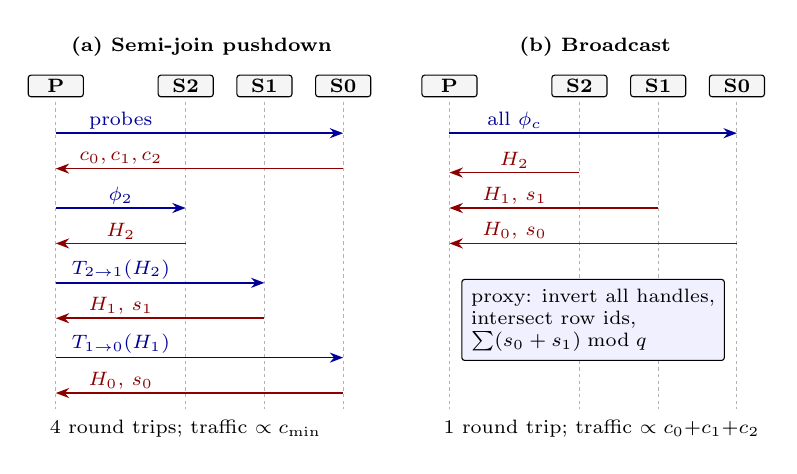
\begin{tikzpicture}[font=\scriptsize, >={Stealth[length=1.7mm]},
  life/.style={draw=gray!60, thin, dash pattern=on 1.2pt off 1.2pt},
  msg/.style={->, semithick, blue!60!black},
  ret/.style={->, semithick, red!55!black},
  ml/.style={anchor=south, inner sep=1.2pt, text=blue!60!black},
  rl/.style={anchor=south, inner sep=1.2pt, text=red!55!black},
  head/.style={draw, fill=gray!8, rounded corners=1pt, minimum width=7mm, inner sep=1.5pt, font=\scriptsize\bfseries}]
\newcommand{\lanes}[1]{%
  \foreach \n/\x in {P/0, S2/1.65, S1/2.65, S0/3.65} {\node[head] at (\x,0) {\n}; \draw[life] (\x,-0.2) -- (\x,-#1);}}
\newcommand{\lbl}[3]{\node[#1] at (0.825,#2) {#3};}
% ---- (a) pushdown
\begin{scope}
\node at (1.85,0.5) {\textbf{(a) Semi-join pushdown}};
\lanes{4.1}
\draw[msg] (0,-0.6) -- (3.65,-0.6);   \lbl{ml}{-0.6}{probes}
\draw[ret] (3.65,-1.05) -- (0,-1.05); \lbl{rl}{-1.05}{$c_0,c_1,c_2$}
\draw[msg] (0,-1.55) -- (1.65,-1.55); \lbl{ml}{-1.55}{$\phi_2$}
\draw[ret] (1.65,-2.0) -- (0,-2.0);   \lbl{rl}{-2.0}{$H_2$}
\draw[msg] (0,-2.5) -- (2.65,-2.5);   \lbl{ml}{-2.5}{$T_{2\to1}(H_2)$}
\draw[ret] (2.65,-2.95) -- (0,-2.95); \lbl{rl}{-2.95}{$H_1,\,s_1$}
\draw[msg] (0,-3.45) -- (3.65,-3.45); \lbl{ml}{-3.45}{$T_{1\to0}(H_1)$}
\draw[ret] (3.65,-3.9) -- (0,-3.9);   \lbl{rl}{-3.9}{$H_0,\,s_0$}
\node[anchor=west] at (-0.2,-4.35) {4 round trips; traffic $\propto c_{\min}$};
\end{scope}
% ---- (b) broadcast
\begin{scope}[xshift=50mm]
\node at (1.85,0.5) {\textbf{(b) Broadcast}};
\lanes{4.1}
\draw[msg] (0,-0.6) -- (3.65,-0.6);   \lbl{ml}{-0.6}{all $\phi_c$}
\draw[ret] (1.65,-1.1) -- (0,-1.1);   \lbl{rl}{-1.1}{$H_2$}
\draw[ret] (2.65,-1.55) -- (0,-1.55); \lbl{rl}{-1.55}{$H_1,\,s_1$}
\draw[ret] (3.65,-2.0) -- (0,-2.0);   \lbl{rl}{-2.0}{$H_0,\,s_0$}
\node[draw, rounded corners=1pt, fill=blue!6, align=left, anchor=north west, font=\scriptsize] at (0.15,-2.45)
  {proxy: invert all handles,\\ intersect row ids,\\ $\sum (s_0+s_1) \bmod q$};
\node[anchor=west] at (-0.2,-4.35) {1 round trip; traffic $\propto c_0{+}c_1{+}c_2$};
\end{scope}
\end{tikzpicture}
}
\caption{Message flow of query Q4 under (a) pushdown and (b) broadcast.}
\label{fig:seq}
\end{figure}

% =====================================================================
\section{Implementation}\label{sec:impl}
We wrote \sys{} and all baselines except SCQL in Python~3.12. The code, the data loaders, and the scripts that produce each table and figure of this paper are available at \url{https://github.com/shivsegv/zs_prism}. AES, AES-GCM \cite{nist80038d}, HMAC and HKDF are taken from the \texttt{cryptography} package, which uses OpenSSL. For Paillier we use \texttt{python-paillier} with \texttt{gmpy2}. Random values come from the OS CSPRNG. A provider is an OS process with an in-memory SQLite~3.53 database, in which each predicate column has a secondary index. It communicates over TCP using MessagePack frames that carry a length prefix and a CRC-32 checksum. Results are sent as packed columns of 16-byte handles and 64-bit shares. To translate a candidate set, the proxy makes a single AES call for the whole set, and the semi-joins are executed by SQLite at the providers. The network is emulated at the server. When a request has been processed, the server delays the reply by the configured RTT plus the time its bytes would take at the configured rate. The latencies we report consist of this network time and the actual cost of encoding, sockets and the database.

\textbf{Baselines.} SCQL runs in its own deployment. The other baselines use our harness and its network emulation. \emph{Map split} has the placement, shares and executor of \sys{}. Its handles are independent random 128-bit values, one per provider, and the proxy maintains a forward and a reverse map. We implement the maps as hash maps for writes and add a sorted-array index for vectorized lookups, so that map split benefits from the packed data path as well. It stands for the design in the survey where linkage is stored at the proxy \cite{domingo2019survey}. \emph{Shared-TID split} stores the same identifier at every provider \cite{aggarwal2005two}. As both run the adaptive executor, the three split systems are identical except for linkage. \emph{DET+Paillier} corresponds to the DET and HOM layers of CryptDB with one provider \cite{popa2011cryptdb}. Every attribute has an HMAC equality tag. A range over the small age domain is rewritten as a list of tags. A SQL aggregate at the provider multiplies Paillier ciphertexts (2048-bit modulus), and each record is additionally stored under AES-GCM. \emph{DET+AEAD} differs only in the aggregate: it retrieves the AES-GCM records that match and processes them at the proxy, in the style of Hacig\"um\"u\c{s} \emph{et al.} \cite{hacigumus2002executing}. \emph{AEAD scan} keeps only AES-GCM records, and the proxy decrypts the full table for each query. \emph{3PC-RSS} is our stand-in for current MPC analytics \cite{bogdanov2008sharemind,liagouris2023secrecy,poddar2021senate}. \emph{All} attributes are held by three servers as replicated additive and XOR shares, in the semi-honest model with an honest majority. A predicate is a Boolean circuit over bit-sliced shares, with an AND tree of logarithmic depth for equality and a Hillis--Steele prefix comparator for ranges. The result bits are converted into arithmetic shares over $\mathbb{Z}_{2^{64}}$, and the servers open nothing except the aggregate or the selected record. For each layer of AND gates or multiplications, the three server processes exchange one round of messages in a ring, and they generate correlated randomness by AES-CTR zero-sharing. The servers see the query and $N$ and nothing else, so we use 3PC-RSS to show what it costs to hide everything. Finally, we run \emph{SecretFlow-SCQL} \cite{fang2024scql} in version 1.0.0b1 from the published image. The deployment is that of its centralized tutorial, with an SCDB server as coordinator, one engine for each party, and MySQL. The table is split vertically between two parties. Party alice has \texttt{id, age, sex, hours} and party bob has the other attributes. We set the Column Control Lists as in the tutorial. A party may read its own columns. The other party may see join keys once the PSI join has run, the outcomes of comparisons, and aggregates. SCQL's own evaluation emulates a wide-area network with \texttt{tc netem}, and we do the same on the link between the two engines. The anonymization baselines are MDAV heterogeneous microaggregation \cite{domingo2005ordinal} and Mondrian \cite{lefevre2006mondrian}, both applied to the six QIs.

% =====================================================================
\section{Evaluation}\label{sec:eval}
\textbf{Setup.} All experiments were run on an Apple M4 with 10 cores and 24\,GB of RAM under macOS. From Adult we take the train and test parts and drop records with missing values, which leaves \NAdult{} records. For larger sizes we draw $2\times10^5$ and $10^6$ records from it with replacement. The second data set is UCI Census-Income (KDD) \cite{census2000}. We use all of its 299,285 records, with the attributes and fragments chosen as for Adult and weeks worked as the measure. The workloads are given in Table~\ref{tab:workloads}. For the local experiments we build three independent instances with new keys and samples, warm each one up, and time 11 repetitions. WAN and SCQL experiments have five repetitions, and SCQL at $10^6$ records has three. All reported values are medians. Among the split-system measurements above 1\,ms, 95\% have an interquartile range within \MaxIQR{} of the median. Before a query is timed, its answer is compared with a plaintext evaluation, and the run stops if they differ.

\begin{table}[t]
\centering
\caption{Workloads on Adult (selectivity at $N=45{,}222$).}
\label{tab:workloads}
\scriptsize
\setlength{\tabcolsep}{3pt}
\begin{tabular}{@{}llr@{}}
\toprule
ID & Query & Rows\\
\midrule
Q1 & full record by identifier (reassembled from $S_0,S_1,S_2$) & 1\\
Q2 & \texttt{COUNT} where \texttt{occupation}=Prof-specialty ($S_2$ only) & \SelQtwo\\
Q3 & \texttt{AVG(hours)} where \texttt{age} $\in[30,45]$ & \SelQthree\\
Q4 & Q3 $\wedge$ \texttt{education}=Bachelors $\wedge$ \texttt{occupation}=Exec-managerial & \SelQfour\\
Q5 & \texttt{age}$\in[70,75]\wedge$Female$\wedge$Widowed$\wedge$United-States & \SelQfive\\
\bottomrule
\end{tabular}
\end{table}

\subsection{Correctness}
We test each system differentially against a plaintext reference. A test consists of \CorrQueries{} random conjunctive \texttt{COUNT}/\texttt{AVG} queries on one to four attributes, mixed with updates, deletions, insertions and lookups of full records. For DET+Paillier and the AEAD scan we use 300 queries. \sys{} is tested once for each of its three plans. In all tests every answer is identical to the reference. For averages we compare the count and the sum, so no rounding is involved.

\subsection{C1: Proxy state and failover}
Fig.~\ref{fig:state} shows what the linkage map costs and what \sys{} needs in its place. Panel (a) plots the persistent linkage state. Panel (b) plots how long a new replica needs until it can answer cross-fragment queries. One map entry consists of a 12-byte row identifier and three 16-byte handles. This gives 60 bytes per record in the most compact encoding. Held in memory as a hash map, an entry takes \MapHeapPerRec{} bytes. With $10^6$ records, a proxy replica that starts or recovers has to fetch 60\,MB and needs \MapBootMillion{} to rebuild the maps, and only then can it answer a cross-fragment query. With $3\times10^6$ records the rebuild takes \MapBootThree{}. A \sys{} replica reads 32 bytes and derives the two subkeys, which takes \ZSBoot{}. In a real deployment the map would cost more than we measured, because replicas that insert concurrently also have to keep their maps consistent. \sys{} replicas only have $K$ in common.

\begin{figure}[t]
\centering
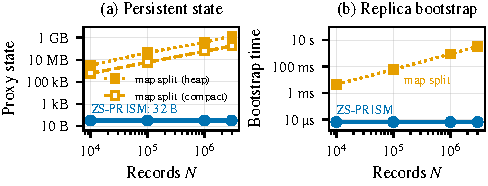
\includegraphics[width=\columnwidth]{state.pdf}
\caption{Proxy linkage state (a) and replica recovery time (b).}
\label{fig:state}
\end{figure}

\subsection{Local performance}
Table~\ref{tab:local} lists ingestion throughput and query latency on loopback. Each value is the median of three instances. Removing the map did not make \sys{} measurably slower. \sys{} \LocalSlowerClause{} map split on any workload, and on joins it is up to \LocalFaster{} faster. Its ingestion rate is also higher, \IngZS{} records/s compared with \IngMap{}. The reason is that \sys{} computes the three handles of a batch in one AES call, whereas map split has to generate three random keys per record and insert them into its index. On conjunctive queries the two DET designs are the fastest systems, since the complete predicate is evaluated by a single provider. This provider, however, holds the equality tags of all QIs side by side. It can therefore compute joint frequencies, and keeping those from a provider is the purpose of splitting \cite{naveed2015inference}. With homomorphic aggregation the provider does not see the measure. On an aggregate over many rows such as Q3, it must multiply thousands of 4096-bit ciphertexts and is slower than the split systems. Ingestion with Paillier reaches \IngPaillier{} records/s and is \PaillierSlowdown{} slower than \sys{}. 3PC-RSS evaluates bit-sliced circuits at memory bandwidth. On a single host this makes it faster than \sys{} for broad aggregates (Q4: \MPCLocalQfour{} vs.\ \ZSLocalQfour{}). Its running time is proportional to $N$ and does not depend on selectivity, so a point lookup at $10^6$ records takes \MPCLookupMillion{}, while \sys{} needs \ZSLookupMillion{}. For $10^6$ records, \sys{} ingests the data in \MillionIngZS{} and answers Q4 in \MillionQfourZS{}. The AEAD scan needs \MillionScan{} for a query at this size. The anonymized releases are fast to query, but the answers contain errors. Over 1,000 random queries, the median error of \texttt{COUNT} at $k=5$ is \UtilMdavFive{} with MDAV and \UtilMondFive{} with Mondrian. At $k=50$, \UtilMondTail{} of the Mondrian answers deviate by more than 10\%. The split systems return exact answers. What they reveal are the marginal distributions of the QIs stored in clear.

\begin{table}[t]
\centering
\caption{Ingestion throughput and median latency (ms), loopback, $N=45{,}222$.}
\label{tab:local}
\scriptsize
\setlength{\tabcolsep}{2.4pt}
\begin{tabular}{@{}lrrrrrr@{}}
\toprule
System & rec/s & Q1 & Q2 & Q3 & Q4 & Q5\\
\midrule
\textbf{\sys{}} & 113{,}192 & 0.20 & 0.15 & 25.0 & 7.81 & 5.35\\
Map split & 90{,}480 & 0.16 & 0.15 & 28.4 & 9.18 & 5.41\\
Shared-TID split & 116{,}427 & 0.18 & 0.15 & 22.6 & 6.09 & 5.19\\
\midrule
DET+Paillier & 220 & 0.08 & 0.12 & 83.1 & 6.38 & 6.49\\
DET+AEAD & 56{,}868 & 0.08 & 0.15 & 24.7 & 2.09 & 3.42\\
AEAD scan & 368{,}585 & 61.6 & 71.6 & 68.4 & 79.6 & 69.0\\
3PC-RSS & 617{,}591 & 12.4 & 1.88 & 3.09 & 3.51 & 3.53\\
\bottomrule
\end{tabular}

\end{table}

\subsection{C3: Selectivity ordering and wide-area execution}\label{sec:wan}
We first look at the amount of data. For Q4, pushdown transfers \PDKBQfour{} per query and broadcast \BCKBQfour{}. For Q5 the numbers are \PDKBQfive{} and \BCKBQfive{}. Pushdown thus sends \PDSaveQfour{} and \PDSaveQfive{} less, as it forwards only the smallest candidate set. Whether this compensates for the additional round trips depends on the link. In Fig.~\ref{fig:wan} we vary the RTT between 1 and 50\,ms for link rates of 100\,Mb/s and 1\,Gb/s. The curve labelled ZS-PRISM is the adaptive executor. Pushdown and broadcast are the same system restricted to one plan. Each of the fixed plans is the better one in part of the range. For small RTTs pushdown is ahead, and more so when the link is slow (Q4, 100\,Mb/s, 1\,ms: \WanPDlow{} vs.\ \WanBClow{}). For large RTTs broadcast is ahead (Q4, 1\,Gb/s, 50\,ms: \WanBChigh{} vs.\ \WanPDhigh{}). We compared the adaptive executor with the better fixed plan at every combination of RTT, rate and query for Q3--Q5. In \WanAutoBestFrac{} cases it is faster or at most 5\% slower, and its largest disadvantage is \WanRegretMax{}. Q5 contains one very selective predicate. Here the adaptive executor is \WanAdaptiveWin{} faster than both fixed plans at 100\,Mb/s and 10\,ms. The small results are returned with the probe, and only the large one has to be completed by pushdown. The median difference between Shared-TID splitting and \sys{} is \WanSharedDiff{}, which shows that the time to derive handles hardly matters. Map split is slower by up to \WanMapWorse{}. Its translation is more expensive, and the planner then selects a different plan. The designs with a single provider complete a query in one round trip, so for selective queries they are the fastest at high RTT. The AEAD scan has to transfer the encrypted table and takes \WanScan{} per query. For Q4, 3PC-RSS requires \MPCRounds{} rounds. At 10\,ms this amounts to \MPCQfourTen{}, compared with \ZSQfourTen{} for \sys{}.

\begin{figure*}[t]
\centering
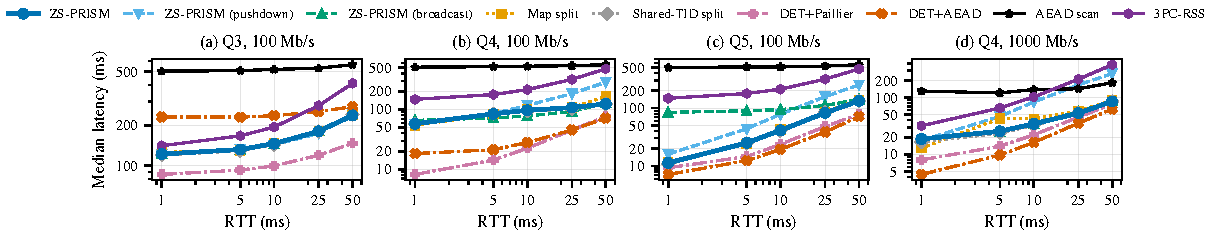
\includegraphics[width=\textwidth]{wan.pdf}
\caption{Median latency under emulated wide-area links (log scales).}
\label{fig:wan}
\end{figure*}

\subsection{Second data set: Census-Income}
We repeated the comparison on the 299,285 Census records (Table~\ref{tab:census}). The queries are analogous to Q1--Q5. The column ``Rand.'' is the median latency of 200 random queries. All answers were verified. On loopback, \sys{} \CensusSlowerClause{} map split on any workload, and on joins it is up to \CensusFaster{} faster. On one host DET+AEAD is again the fastest system for selective queries, for which it stores all equality tags at one provider, and 3PC-RSS is the fastest for the broad range aggregate Q3. With an RTT of 10\,ms, 3PC-RSS is slowed down by its rounds and the AEAD scan by the transfer of all records. The order of the systems is the same as on Adult.

\begin{table}[t]
\centering
\caption{Census-Income ($N=299{,}285$): median latency (ms).}
\label{tab:census}
\scriptsize
\setlength{\tabcolsep}{2.2pt}
\begin{tabular}{@{}lrrrrrrr@{}}
\toprule
 & \multicolumn{4}{c}{loopback} & \multicolumn{3}{c}{10\,ms, 100\,Mb/s}\\
\cmidrule(lr){2-5}\cmidrule(l){6-8}
System & Q1 & Q3 & Q4 & Rand. & Q1 & Q4 & Rand.\\
\midrule
\textbf{\sys{}} & 0.20 & 121 & 26.7 & 6.13 & 25.7 & 185 & 45.9\\
Map split & 0.20 & 140 & 36.0 & 6.49 & 25.4 & 184 & 49.1\\
Shared-TID split & 0.21 & 105 & 21.3 & 5.45 & 25.4 & 182 & 44.9\\
DET+AEAD & 0.09 & 118 & 10.2 & 2.08 & 12.7 & 71.2 & 16.7\\
AEAD scan & 484 & 594 & 605 & 603 & 3698 & 3810 & 3829\\
3PC-RSS & 69.1 & 23.8 & 27.0 & 18.9 & 2415 & 879 & 659\\
\bottomrule
\end{tabular}

\end{table}

\subsection{Comparison with recent systems}\label{sec:sota}
\textbf{SecretFlow-SCQL, measured.} For Table~\ref{tab:scql} we loaded the same records into SCQL and into the split designs and ran the same queries. The network is the WAN setting of the SCQL paper, 100\,Mb/s with an RTT of 20\,ms. Between the SCQL engines we measured \ScqlRtt{}. Q4 and Q5 are conjunctions across both parties, and \sys{} answers them \ScqlSpeedupMin{}--\ScqlSpeedupMax{} faster than SCQL. For Q4 the latencies are \ZSQfourWanA{} and \ScqlQfourWanA{} on Adult and \EightZSQfourWan{} and \ScqlQfourWanM{} at $10^6$ records. Without network delay SCQL takes \ScqlQfourLocA{} and \ScqlQfourLocM{} for Q4. For Q3 the result is reversed. In SCQL the party that stores \texttt{age} also stores \texttt{hours} in clear, so it can answer Q3 by itself, in \ScqlQthreeWanM{} at $10^6$ records. In \sys{} the measure is not available to any provider (C2). The proxy has to fetch shares from two providers over the WAN, and Q3 takes \ZSQthreeWanM{}. The two systems do not protect the same things. With the CCL we configured, the other party in SCQL learns join keys and the outcomes of predicates and does not learn the measure. A provider in \sys{} learns its own columns and its query traces. It learns neither the identifier nor the measure.

\begin{table}[t]
\centering
\caption{SecretFlow-SCQL versus split designs: median latency (ms), 100\,Mb/s, 20\,ms RTT.}
\label{tab:scql}
\scriptsize
\setlength{\tabcolsep}{3pt}
\begin{tabular}{@{}lrrrrrr@{}}
\toprule
 & \multicolumn{3}{c}{Adult} & \multicolumn{3}{c}{$10^6$ records}\\
\cmidrule(lr){2-4}\cmidrule(l){5-7}
System & Q3 & Q4 & Q5 & Q3 & Q4 & Q5\\
\midrule
SCQL 1.0 (measured) & 11.0 & 755 & 585 & 103 & 2078 & 929\\
\textbf{\sys{}} & 155 & 86.4 & 63.0 & 2189 & 911 & 212\\
Map split & 153 & 119 & 61.8 & 2314 & 971 & 285\\
3PC-RSS & 249 & 277 & 280 & 2581 & 2689 & 2700\\
\bottomrule
\end{tabular}

\end{table}

\textbf{Published results.} For S$^2$ the authors report roughly 1.5\,s for a conjunctive search over $10^6$ rows, including retrieval of the rows, within one AWS region \cite{sharma2023s2}. On a link of 1\,Gb/s and 1\,ms, which is similar, \sys{} takes \EightZSQfourLan{} for Q4. HE$^3$DB is reported to need 241\,s for a single TPC-H query over $10^4$ rows \cite{bian2023he3db}. The queries and the hardware differ from ours, so these values should be read as orders of magnitude. It should also be kept in mind that both systems give stronger guarantees. S$^2$ does not reveal which or how many rows match, and under FHE the server learns nothing.

\subsection{C2: Writes with dual-share refresh}
An update writes the two new shares in parallel. The differential tests verify the answers after each update. On loopback an update, a deletion and the insertion of one record take \WriteZS{}\,ms in \sys{}. The other split designs need the same time, which means that the refresh of the second share does not add a round trip. At 10\,ms RTT the three operations need two, two and one round trips. An update in DET+Paillier takes \WritePaillier{}\,ms, as the new value has to be encrypted.

\subsection{What \sys{} does not hide: collusion attacks}\label{sec:attacks}
\textbf{Snapshots.} In the first attack $S_0$ and $S_2$ combine their complete tables. With Shared-TID splitting an equality join links \SnapShared{} of the records. With \sys{} and with map split the join links \SnapZS{}, and aligning the two tables by storage order links \SnapRankZS{}. This agrees with Proposition~1. For the share holders $S_0$ and $S_1$ the situation is different. In each of the split systems they can test whether $s_0+s_1\bmod q\in[1,99]$, which takes $O(N\log N)$ time and links \SnapShareSum{} of the records. The protection of the measure therefore relies on the assumption that these two providers do not collude.

\textbf{Query traces.} A provider also sees the handles in its requests and replies. Within one query, each candidate list contains only rows from earlier results. Two colluding providers can collect such constraints over many queries and intersect them. We ran this intersection attack against 1,000 target records on Adult with up to 1,000 random queries (Fig.~\ref{fig:attack}). Panel (a) gives the number of targets for which exactly one partner remains. Panel (b) gives the median number of remaining candidate partners, and the dotted line at $N=45{,}222$ corresponds to an attacker who has learned nothing. Pushdown passes candidate lists from one provider to the next. With this plan the colluding pairs $S_0+S_2$ and $S_1+S_2$ link \TraceLinkedPD{} of the targets exactly, and the median candidate set falls from 45,222 to \TraceSetPD{}. With broadcast the providers return results and receive no candidates. In that case \TraceBCClause{}, and the median candidate set remains at \TraceSetBC{}. An operator can thus reduce trace leakage by enforcing broadcast and pays for it with the latencies in Fig.~\ref{fig:wan}. To remove the leakage altogether one would have to use ORAM \cite{stefanov2013path}, secret sharing that hides access patterns \cite{sharma2023s2}, or MPC \cite{liagouris2023secrecy}.

\begin{figure}[t]
\centering
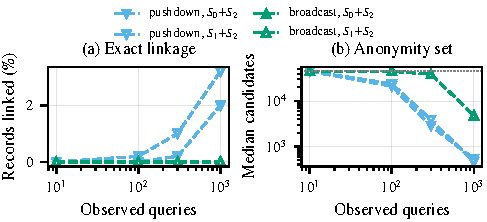
\includegraphics[width=\columnwidth]{attack.pdf}
\caption{Query-trace intersection attack by two colluding providers.}
\label{fig:attack}
\end{figure}

% =====================================================================
\section{Discussion and Limitations}\label{sec:disc}
\textbf{Security scope.} The guarantee of \sys{} concerns the linkage of stored fragments. It does not cover predicates, result sizes or access patterns. It also assumes that the share holders do not collude, and over time the traces reveal part of the linkage. Since the tokens are deterministic, $S_0$ can tell when two identifiers are equal, which is true of every design that supports equality search \cite{bellare2007det}. Proposition~1 says that the handles do not add linkage \emph{beyond} what the clear columns already allow. Attributes that are correlated, for example \texttt{marital}=Widowed and a high \texttt{age}, permit statistical linkage. This is determined by the fragmentation, and fragmentation methods that account for dependencies deal with it \cite{decapitani2014dependencies}. If $K$ is compromised, the attacker obtains the linkage and can test identifier tokens. The measure is still protected, because it is secret-shared. To replace $K$, each provider rewrites its handle column, which is a linear pass that the providers can run in parallel.

\textbf{Observations.} Two results differed from what we had assumed at the start. We thought that giving up the map would slow down local execution somewhat. This was not the case, and ingestion became faster, for the reason given in Section~\ref{sec:eval}. We also had not expected the query plan to influence privacy. Because pushdown hands candidate lists from provider to provider, its traces contain more linkage information than those of broadcast.

\textbf{Evaluation scope.} All providers ran on the same machine and the network delay was emulated. We did not deploy across different clouds. Our systems are written in Python, and a compiled implementation would have lower absolute latencies. SCQL has an advantage in our comparison, as it is compiled C++ and we did not delay its coordinator links. The 3PC baseline is semi-honest. Optimized engines \cite{liagouris2023secrecy,poddar2021senate} compute faster, but they need the same number of rounds, and at wide-area RTTs the rounds dominate. We leave constraint-driven fragmentation \cite{ciriani2010combining}, dependency-aware placement \cite{decapitani2014dependencies} and execution that hides traces to future work.

% =====================================================================
\section{Conclusion}
Splitting systems so far either stored a common identifier in all fragments, which two providers can join on, or kept a linkage map at the proxy whose size grows with the data. In \sys{} a handle is the encryption of a random row identifier and the provider index under a key known only to the proxy. Handles at different providers cannot be linked, the proxy can invert them, and its persistent state is 32 bytes. In combination with dual-share splitting and selectivity-ordered sequential execution, the system returns exact answers about as fast as a map-based design, and a failed proxy is replaced by loading one key. Our attacks show the remaining leakage, which comes from colluding share holders and from query traces. As next steps we want to lower the trace leakage without losing index-based execution, and to run the experiments with providers in separate clouds.

\bibliographystyle{IEEEtran}
\bibliography{refs}

\end{document}
